\section{Implementation}
\label{sec:impl}

%We have implemented a complete prototype system, which provides basic functions of a distributed reliable backup storage system, including data deduplication, file chunk distribution control, file data upload/download, fault tolerance by erasure codes and etc.
%\textbf{Overview \& Components} 

We implement a distributed storage system prototype that realizes
deduplication and erasure coding and supports different data placement
policies including the baseline (see Section~\ref{sec:motivate}), EDP, and
CEDP.  Figure~\ref{fig:prototype} shows the system architecture, which 
comprises three main components: one or multiple clients, a metadata server,
and multiple storage nodes.  

\begin{figure}[H]
\centering
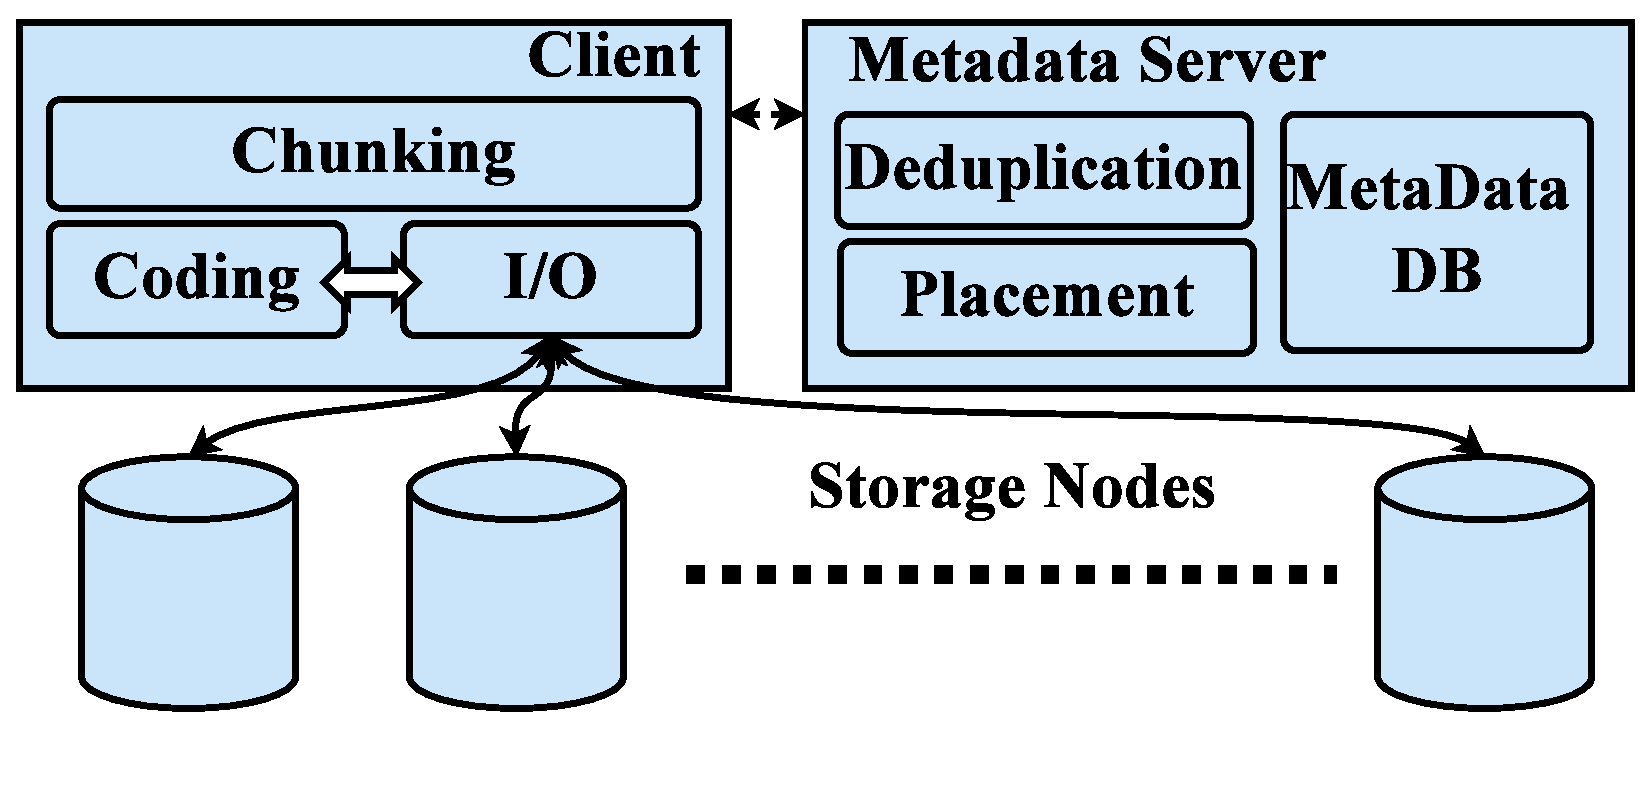
\includegraphics[width=\linewidth]{system_overview.eps}
\vspace{-15pt}
\caption{Architectural overview of our prototype.}
\label{fig:prototype}
\vspace{-6pt}
\end{figure}

File writes operate on a per-batch basis (see Section~\ref{subsec:p_form}).
Specifically, a client divides files into chunks and computes the
fingerprints.  For each batch of chunks to be written, the client sends the
fingerprints to the metadata server, which performs deduplication and runs the
data placement policy (e.g., the baseline, EDP, or CEDP).  The metadata server
also maintains the file metadata to keep track of chunks associated with a
file.  It then responds to the client with the list of unique chunks and how
they are placed across nodes.  The client then applies erasure coding to the
unique chunks, and writes the encoded chunks to different nodes in parallel. 

%batch, we group every $k$ unique chunks that are assigned to $k$ distinct
%nodes as the data chunks of a stripe. We then generate additionally $n-k$
%parity chunks and place them on $n-k$ other distinct nodes.

%For each group of $k$ 
%data chunks, we assign the $n-k$ parity chunks onto $n-k$ {\color{red}
%out of $N-k$} other distinct nodes.  We rotate the $n-k$
%nodes for parity chunks over all the permutations of $n-k$ out of $N-k$ nodes
%across different batches of chunks to balance the parity load.  We consider
%the number of unique chunks in a batch that is equal to the number of data
%chunks of the stripes that and the resulting batch size is ${N \choose n}
%\times n \times k$, with $C$ equal to ${N \choose n}\times n \times k / N$.} 

File reads operate in the reverse way.  To read a file, the client queries the
metadata server for all required chunks of a file.  It then reads all chunks
from the nodes in parallel. In the presence of node failures, the client
issues degraded reads to retrieve $k$ data and parity chunks from other
surviving nodes to decode the unavailable chunks. 

To integrate with erasure coding, we group every $k$ unique chunks as the data
chunks of a stripe.  To balance the distribution of parity chunks, we
enumerate all ${N\choose n}$ possible stripe permutations and $n$ possible
parity rotations.  Thus, the resulting batch size is 
$N\times C = {N\choose n}\times n \times k$ data chunks.  We pick $C$
accordingly given $N$, $n$, and $k$. 

%A client can initiate either file upload or download request. 
%To upload files, the client divides them into chunks, and, then, sends metadata of the chunks to metadata server. 
%On receiving response from metadata server, the client encodes the data chunks, and uploads each coded chunk to its destination storage node.
%After encoding, the client distributes each code chunk to its targeted storage slave.
%To download a file, the client queries the metadata server about all the required chunks to reconstruct the original file, and establishes connections with all the storage nodes to download these chunks concurrently.

%The metadata server is mainly responsible for handling clients' requests and managing persistent metadata for future requests. 
%In response to an upload request, the metadata server should inform the client of which chunks of the uploaded files are unique, as well as on which slaves these unique chunks should be stored.
%At the meantime, the metadata server records all the chunks, either duplicate or unique, of the uploaded files and their residing slaves in local metadata files.
%The metadata server will utilize these metadata files to handle clients's download requests so that the clients know how to reconstruct their uploaded files.

%The task of a storage slave is straightforward: it stores chunks from clients to local disk, and sends back stored chunks to clients whenever they request for them.



%\textbf{Pipelined multi-threading} 
%Each component internally consists of several services or layers, and these services or layers are implemented as threads in the implementation.
%\subsection{Client}
%\begin{itemize}
%\item \emph{Chunking}
%\item \emph{Coding}
%\item \emph{Data Transmission}
%\end{itemize}
%\textbf{Scalability \& Tools} 
%For scalability, we shift data-oriented computation-intensive tasks, including chunking, hashing and erasure coding, to the client.
%In file upload, the client locally chunks the files, using either fixed-size chunking or variable-size chunking via Rabin-fingerpint, and sends only necessary metadata of each chunk to metadata server.
%The coding layer encodes or decodes chunks of data using Reed-Soloman Codes, provided by the Jerasure2.0 \cite{pg:14:jer} library with GF-Complete \cite{pmg:13:gfc10}.

%For perfect parallel data accesses, in either upload or download operation,
%the client creates a group of threads, each of which persistently
%connects with a storage node, for data transmission to or from the
%storage nodes.  To avoid downloading duplicate chunks of a file multiple
%times, in file download operation, the client maintains a bitmap to
%record the chunks that have been donwloaded, and, if a chunks has been
%downloaded before, the client reads it either from local download cache
%or the downloaded file without network transmission.

To improve disk I/O efficiency, each storage node organizes data in 
{\em containers} \cite{zhu08}, which serve as disk read/write units.  We now
configure each container to keep at most 64 chunks.  When a node writes a
chunk, it first appends the chunk to an in-memory container, which is flushed
to disk when it is full.  To read a chunk, the node reads the corresponding
container as a whole into the local cache and retrieves the chunk. 

%For each chunk, in addition to identifying whether it is unique or duplicate,
%the prototype needs to know where the existing chunk resides if the chunk
%is duplicate. We add 1 byte, i.e. covering maximum 256 storage nodes, to
%the value field of each entry of a unique chunk indexed by its
%fingerprint in the fingerprint index. Thus, one single index lookup can
%handle queries for both deduplication and EDP.

We implement our prototype in C, and realize some operations using open-source
libraries.  We choose and implement 160-bit SHA-1 as fingerprints for
deduplication using OpenSSL \cite{openssl}.  We also choose and implement
Reed-Solomon coding \cite{reed60} as our erasure coding scheme using
Jerasure~2.0 \cite{pg:14:jer} and GF-Complete \cite{pmg:13:gfc10}.  In the
metadata server, we maintain metadata in key-value databases and implement
them using the Kyoto Cabinet library \cite{kyotocab}. 

%Our current prototype only implements fixed-size chunking, while we address
%the workloads with variable-size chunks using simulations (see
%Section~\ref{sec:evaluation}).  


%The metadata server requires two hash maps, the \textit{chunk hash index} and
%the \textit{chunk-node index}, for deduplication and balancing chunk
%distribution, respectively, and it uses two fixed-size in-memory hash indices
%backended by on-disk full indices, based on Kyoto Cabinet file hash database
%\cite{kyotocab}, for these purposes.  The chunk distribution hash map maps
%the chunk ID of a duplicate chunk to its residing storage node ID, and the
%distribution service utilizes this map to get $d_{i,j}$, the number of
%duplicate chunks of $i$-th file on the $j$-th storage node.

%The chunking module at client side has two modes: i) variable-size chunking; ii) fixed-size chunking.
%For variable-size chunking, the chunking module utilizes Rabin-fingerprint to efficiently chunk the files.
%And we use the SHA1 function of OpenSSL library~\cite{openssl} to calculate a 20 bytes' hash for each chunk.
%For real file data upload, we adopt rabin-fingerprint-based variable-size chunking. 
%Basically, this type of chunking yields higher deduplication ratio than fixed-size chunking does. 
%For backup trace, the trace itself consists of all the hashes, as well as some other metadata, of pre-chunked data while the raw data is not available.
%In this case, the client uses the hashes in the trace, either directly or by calculating a super-hash with hashes of several chunks, for upload request.
%The coding service consists of a single thread for either encoding or decoding. 
%In file upload operation, once response on where to distribute each unique chunk is received, the coding service reads unique chunks belonging to the same stripe into memory, calculates the parity chunks and distributes both data chunks and parity chunks to the data IO layer.
%In file download operation, if a chunk can not be downloaded from a slave, the client will informs the data IO layer to download other chunks belonging to the same stripe from other alive slaves, and downloaded chunks will be dispatched to the coding service.
%With sufficient data, the coding service reconstructs the needed chunk and writes it to local file.
%Currently, our prototype supports Reed-Solomon Codes only, and our implementation of the coding service is based on Jerasure2.0~\cite{pg:14:jer} with GF-Complete~\cite{pmg:13:gfc10}.
%The data IO layer is actually a group of threads, each of which is connected with one of the storage slaves.
%For file upload, each IO thread is associated with the coding service via a queue.
%For file download, each IO thread receives download request from the communicator via a queue as well.To improve the network transmission efficiency, for either upload or download, the data IO layer packs several data chunks into a large packet before sending them out. 
%The download operation at client is accelerated by a least-recently-used-based chunk cache, with maximum size equal to that of 1024 chunks.

%\subsection{Metadata Server}
%\begin{itemize}
%\item \emph{Deduplication}
%\item \emph{Even Datat Distribution}
%\item \emph{File Recipe}
%\item \emph{Recipe Query}
%\end{itemize}
%\textbf{Tools} 

%At the metadata server side, there are four main modules: i) communicator; ii) deduplication module; iii) distribution module and iv) recipe module, and the four modules are pipelined as a ring, as shown in Figure~\ref{fig:prototype}, to accelerate the processing rate.

%The communicator module receives upload request from client over TCP connection, and sends back response to client using the same connection. 
%As for download request, a RPC service collects information on queried file, and sends the collected information as response.
%The deduplication module utilizes a fixed-sized in-memory hash index backended by an on-disk full index, based on Kyoto Cabinet file hash database~\cite{kyotocab}, to detect whether a chunk is unique or duplicate of an existing chunk.
%If a chunk is duplicate, the deduplication module marks it as duplicate, and passes it on to the next module.
%And for unique chunk, the deduplication module inserts a new record, with the chunk hash as key and its global unique id as value, into the database, mark it as unique and passes it to the next module.

%All the deduplicated chunks are passed to the distribution module.
%The distribution module incorporates the baseline, EDP and CEDP algorithms, and can be switched at the start time of the metadata server.
%The distribution module has a distribution buffer that can buffer ${N \choose n} * n * k$ chunks, where $N$ is the number of storage slaves, $n$ and $k$ are coding stripe size and the number of data chunks in a stripe, respectively.
%While buffering unique chunks in the distribution buffer, the distribution module keeps records of $t$: the number of files involved in the buffer, $U$: the number of unique chunks of each file and $\mathbf{d}$: the number of duplicate chunks of each file on each storage slave.
%These records are necessary for the EDP algorithm to balance the normal reads for each file.
%For each unique chunk, once its destination slave is decided, the distribution algorithm will add a record, with the chunk id as key and the slave id as value, into the chunk-slave map.
%For each stripe of chunks, once the destination slaves for all the chunks are decided, a new entry of stripe metadata, including chunk IDs, residing slaves, and indices of chunks in the stripe, are appended to a local log-structured metadata file.
%These two metadata files not only assist the even data placement algorithm, but also instruct future read operations, either normal or degraded ones.

%The file recipe module records what chunks are necessary to re-construct an uploaded file, as well as how to re-construct the file with these chunks.
%It basically generates a recipe for each uploaded file, and appends an entry, including chunk id, offset and length, for each chunk of the file.

%\subsection{Slave Node}
%\begin{itemize}
%\item \emph{Network Transmission}
%\item \emph{Bucket Disk IO}

%\end{itemize}

%Each slave node is an independent storage agent. 
%Two threads are listening on two pre-configured ports for handling upload and download requests, respectively.
%And, for each new request from client, a worker thread will be created to dedicately handle the request.
%All the communcations, involving either metadata or raw data, with clients are over TCP connections.

%\textbf{Bucket I/O} 
%In addition, each slave has a bucket cache to accelerate the disk read performance, and, due to high spatial locality in backup data, the hit ratio can be quite high.
%Each bucket is of pre-configured size, and, if a bucket can not hold current chunk and the size of the bucket has not reached the pre-configured size, we will pad zeros to the end of the bucket.

%To eliminate overheads in general file system operations, e.g. create, open, close and etc., all buckets on a storage slave is stored in a large, pre-allocated file.
%Each new bucket is appended into the large file, and the offset of a chunk is looked up with its chunk id in the local chunk-offset index.

%\subsection{MetaData}
%\begin{itemize}
%\item \emph{Full Chunk Index}
%\item \emph{Chunk-Slave Map}
%\item \emph{Stripe Log}
%\item \emph{Image Log}
%\item \emph{File Recipe}
%\item \emph{Chunk-Offset Map}
%\item \emph{Bucket Log}
%\end{itemize}
%The metadata server creates several metadata file to assist its services. 
%The \textit{full chunk index} and \textit{chunk-slave index} stores information on key-value mappings.
%Each entry in full chunk index maps chunk hash of 20 bytes to chunk id of 8 bytes while each entry in chunk-slave index maps chunks id of 8 bytes to slave id of 1 byte.
%The full chunk index and chunk-slave index are used in the deduplication and distribution services, respectively.
%Whenever the service starts, part of the index file is load into memory.
%New entries will be synchronized to disk when either the memory consumption reaches pre-set value or the service ends.
%The \textit{stripe log} and \textit{image log} files are log-structured metadata files. 
%The first entry of each file records the number of total entries in the log file.
%Each entry in stripe log file includes stripe id, stripe length, and chunk id and slave id of each chunk, in the order that they appear in the stripe.
%Each entry in the image log file specifies the image id, version number and its size.
%The \textit{file recipe} is created for each uploaded file, and records information on all the chunks of the file.
%For each chunk, its chunk id, offset in the file, its length and its stripe id are recorded.

%Each storage slave maintains the local \textit{chunk-offset index} and \textit{bucket log} metadata.
%The chunk-offset index maps an 8 bytes' chunk id to its 8 bytes' offset in the large local storage file. 
%Once the offset of a chunk is known, the storage slave can calculates id of the bucket that holds the chunk, as well as the offset of the chunk inside the bucket.
%The bucket log records the number of total buckets in the first entry, and, for each bucket, its bucket id, size and last modified time are recorded.
